\chapter{Controlar dispositivos de forma remota}\label{cha:arte}

Existen diferentes alternativas para controlar robots o microcontroladores
de forma remota. Muchas de éstas se agrupan bajo la denominación
``Internet of Things''\footnote{\url{https://www.iotwf.com/resources/1}}.
En este capítulo se describirán algunas iniciativas similares a XRemoteBot.

\section{Educabot}
El proyecto Educabot es una iniciativa de Diego Ramírez con el apoyo de
la Fundación Nahual y la organización
El Galpón del Banquito\footnote{\url{http://minimalart.org/blog/presentando-educabot}}.
Educabot tiene por
objetivo enseñar tecnología a niños y adultos a través
del uso, programación y construcción de robots. En el sitio del proyecto
se ofertan cursos orientados a los distintos niveles y
en la última conferencia de Python de Argentina (PyConAr 2014) uno de
los cofundadores del proyecto mencionó que se llevan adelante actividades
con los robots
en distintas escuelas de la Ciudad Autónoma de Buenos
Aires\footnote{\url{https://youtu.be/1oCOAtX9OS4}}.

% FIXME: ES ORIGINARIO DE ..... EN ESCUELAS? EN ONGS? DONDE SE LOS USA?
% Son cursos privados según dijo el tipo, pero no tengo de donde citar
% eso no dice nada el sitio.
% FIXME: En el sitio no mencionan nada de los cursos en escuelas lo único
% que encontré es lo de youtube que es una charla en la Pycon del fundador

En la parte de construcción de robots, este proyecto plantea un modelo
de robot denominado
``Rolo'' orientado a niños de más de 10 años, mientras que para los más
chicos se plantean actividades con el robot ``elBrian'' que incluyen
controlarlo a través de una interfaz web que muestra las imágenes emitidas
por la cámara incorporada en este robot y además permite controlarlo con
botones en pantalla que determinan en qué dirección debe moverse el robot
(figura~\ref{fig:elbrian}).

\begin{figure}
    \centering
    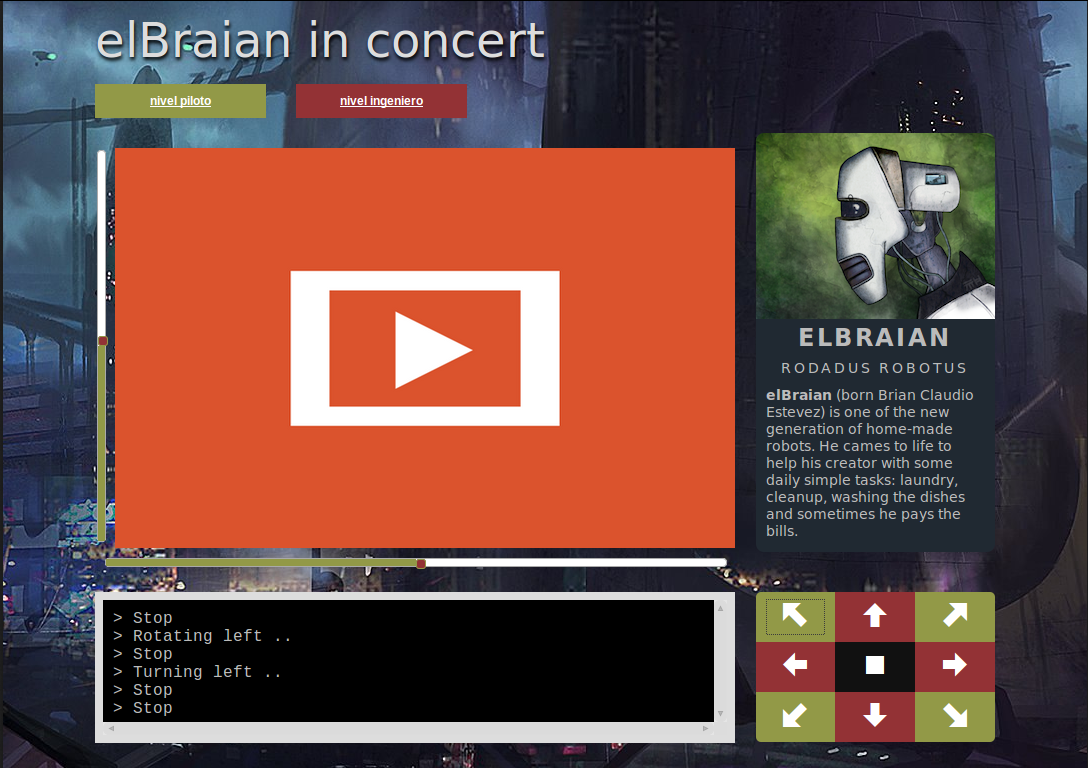
\includegraphics[width=0.5\textwidth]{figures/elbrian-1}
    \caption{Pantalla principal de elBrian (en el recuadro rojo normalmente
        se muestra la cámara de el robot)}
    \label{fig:elbrian}
\end{figure}

Las tecnologías utilizadas en la interfaz web de ``elBrian'' coinciden en gran
parte con las utilizadas en el desarrollo de XRemoteBot, pero el objetivo del
servidor de ``elBrian'' es controlar un único robot en un ambiente local.
Además este servidor
se instala en el robot utilizado,  cuestión que sería imposible en los
robots basados en
microcontroladores AVR y PIC (``Basic Stamp 2`` de Parallax)
a los que XRemoteBot se encuentra dirigido.

%FIXME: fijate de poner aunque sea notas al pie con las referencias de los paquetes o protocolos que nmbras... el que no sabe.. se muere...

El servidor web de ``elBrian'' está implementado usando el framework
Tornado\footnote{\url{http://www.tornadoweb.org/}},
WebSockets\footnote{\url{http://www.websocket.org/}},
mjpg-streamer\footnote{\url{https://github.com/jacksonliam/mjpg-streamer}},
OpenCV\footnote{\url{http://opencv.org/}}
y JSON\footnote{\url{http://json.org/}}.
Este servidor está diseñado para ejecutarse
en el robot ya que el mismo se basa en una placa Raspberry Pi, la cuál
cuenta con un procesador ARM perfectamente capaz de ejecutar un sistema
operativo completo como GNU/Linux y dar soporte al intérprete oficial de
Python.

Mientras que este servidor coincide en gran medida en la elección de lenguaje
y bibliotecas utilizadas, su implementación es específica para el robot ``elBrian''
y no puede ser portada a robots con menores capacidades de procesamiento
sin una reescritura significativa. Además el protocolo utilizado no contempla
el acceso a valores de sensores siendo los únicos mensajes que permite enviar
al robot los comandos de movimientos.

Referencias del proyecto:
\begin{itemize}
    \item Página del proyecto: \url{http://www.educabot.org/}
    \item Código fuente de ``elBrian'': \url{https://github.com/educabot/elBraian}
\end{itemize}

\section{Gobot con cppp-io}

Gobot
es una biblioteca que permite controlar robots programando en el lenguaje
Go\footnote{\url{https://golang.org/}}. Esta biblioteca soporta el
protocolo Firmata
para controlar robots
conectados directamente a través de una interfaz serial, como es el caso
de los robots Multiplo N6, y soporta la API
cppp-io\footnote{\url{https://github.com/hybridgroup/cppp-io/}}
que define una API JSON
que permite el acceso a la información y control de robots a través de la Web.

El proyecto Gobot surge como una iniciativa de la compañía ``The Hybrid Group''.
El objetivo de este proyecto es facilitar la programación de
dispositivos como las placas Arduino y los robots
Sphero
a personas que no sean expertas en la programación de microcontroladores%
\footnote{\url{http://www.wired.com/2015/04/internet-anything-time-everyone-able-hack-robots/}}.


Gobot tiene compatibilidad con distintos sensores y robots, además de
ser compatible con
placas utilizadas normalmente en la construcción de robots como
pueden ser Arduino,
Raspberry Pi, Intel Edison y Beaglebone Black%
\footnote{\url{http://gobot.io/\#platforms}}.

Este proyecto es interesante como base para desarrollar un proyecto
similar a XRemoteBot en Go, pero requiere, además la reimplementación
del módulo de Python DuinoBot que controla, a través de una versión
modificada del protocolo Firmata, a los robots Multiplo N6. Por otro
lado, los robots Scribbler tampoco aparecen en la lista de robots soportados.

Referencias del proyecto:
\begin{itemize}
    \item Página del proyecto: \url{http://gobot.io}.
    \item Protocolo de su API web: \url{https://github.com/hybridgroup/cppp-io/}.
\end{itemize}


\section{Cylon.js}

Cylon.js es un proyecto hermano de Gobot, también es desarrollado
por ``The Hybrid Group'',
y soporta la misma variedad
de dispositivos y también provee una API cppp-io, con la diferencia
de que la biblioteca provista está escrita en Javascript para
``Node.js''\footnote{\url{https://nodejs.org/}}.

Los objetivos de Cylon.js son los mismos que los del proyecto Gobot,
pero trasladados al lenguaje de programación Javascript, en lugar
del lenguaje de programación Go.

Una característica interesante de Cylon.js es que soporta distintos
protocolos para su API remota como ser
HTTP\footnote{\url{http://tools.ietf.org/html/rfc2616}},
socket.io\footnote{\url{http://socket.io/}}
y la capacidad de agregar nuevos protocolos con plugins.

\begin{lstlisting}[caption={Cylon.js controlando 2 robots ``sphero''
usando HTTP (extraído del sitio oficial del proyecto)},
label={lst:cylonjs_ejemplo}]
"use strict";

var Cylon = require("cylon");

// ensure you install the API plugin first:
// $ npm install cylon-api-http
Cylon.api({
  host: "0.0.0.0",
  port: "8080"
});

var bots = {
  "Thelma": "/dev/rfcomm0",
  "Louise": "/dev/rfcomm1"
};

Object.keys(bots).forEach(function(name) {
  var port = bots[name];

  Cylon.robot({
    name: name,

    connections: {
      sphero: { adaptor: "sphero", port: port }
    },

    devices: {
      sphero: { driver: "sphero" }
    },

    work: function(my) {
      every((1).seconds(), function() {
        console.log(my.name);
        my.sphero.setRandomColor();
        my.sphero.roll(60, Math.floor(Math.random() * 360));
      });
    }
  });
});

Cylon.start();
\end{lstlisting}

En el código~\ref{lst:cylonjs_ejemplo} se puede ver un ejemplo de
Cylon.js del lado del servidor exponiendo dos robots de tipo
\textit{sphero} a través de la API HTTP. Los robots sphero son pequeñas
esferas controladas por Bluetooth que pueden desplazarse rotando o
cambiar de color gracias a
leds que iluminan la superficie del robot desde el interior del
mismo\footnote{\url{http://www.gosphero.com}}.

Una vez ejecutado el código~\ref{lst:cylonjs_ejemplo} en el servidor,
a través de la API, se
les podrá enviar un mensaje a los robots que hará que cambien
de color
y se desplacen
rodando.

Si bien en la documentación del proyecto se detalla como habilitar
un sistema de login para acceder a la API de forma remota, el mismo
no parece estar diseñado para el acceso concurrente de distintos usuarios
ya que de la documentación no surge que Cylon.js soporte un sistema
de reserva de robots o de exclusión mutua en el acceso a los mismos.

Referencias del proyecto:
\begin{itemize}
    \item Página del proyecto: \url{http://cylonjs.com/}.
\end{itemize}


\section{VCar}

\begin{figure}
    \centering
    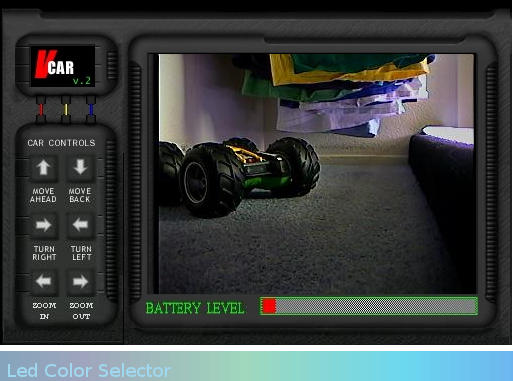
\includegraphics[width=0.5\linewidth]{figures/vcar}
    \caption{Interfaz de VCar}
    \label{fig:vcar}
\end{figure}

VCar es un auto a control remoto, cuyo control fue modificado para
se manipulado por software desde  una computadora con GNU/Linux la
cuál permite controlar el robot de forma remota y verlo
a través de una cámara de
video
(figura~\ref{fig:vcar}).

Este proyecto fue creado por David Mc Anulty con el objetivo de
aprender a ``traducir código en movimientos reales''
(el objetivo no se encuentra
expresado de forma explícita en el sitio web  de VCar, pero se contactó
al autor del proyecto que proporcionó esta información).
Originalmente
este proyecto consistía de un motor paso a paso que permitía mover
una cámara de video de forma remota, eventualmente ante el éxito
del proyecto entre sus amigos, el desarrollador comenzó a investigar
distintas formas de interactuar con la cámara (actualmente se puede
controlar el zoom de la cámara desde la interfaz de VCar) y
finalmente agregó un auto a control remoto similar al que se puede
ver hoy en día en el sitio del proyecto.

La interfaz de VCar posee una botonera que permite mover el robot,
controlar el zoom de la cámara de video y controlar el color
de los LEDs que iluminan al robot.
El acceso al robot es público,
sin ningún tipo de restricción y la página
si bien no tiene detalles de todo el hardware y el software utilizados
provee algunas fotos de la construcción del
sistema\footnote{\url{http://www.hellspark.com/dm/gallery2/v/projects/robotics/vcar/}}.

Referencias del proyecto:
\begin{itemize}
    \item Página del proyecto: \url{http://www.hellspark.com/new/css/vcar/vcar.html}.
    \item Galería de fotos: \url{http://www.hellspark.com/dm/gallery2/v/projects/robotics/vcar/}.
\end{itemize}


\section{Tele Toyland}

Tele Toyland es un sitio que provee acceso a varios dispositivos a través
de una interfaz web. Este proyecto es una iniciativa personal de Carl
Sutter que surgió en 2006 basado en experiencias anteriores, en las que
Sutter participó, como
el primer robot conectado a la web
``Mercury Project''
y ``TeleGarden''~\citep{golberg_2010}.
El objetivo del proyecto es mostrar una serie de dispositivos
creados por el autor del sitio con el fin de inspirar a la gente (especialmente
a chicos) a realizar proyectos similares (el objetivo no se encuentra
expresado de forma explícita en el sitio web  de Tele Toyland, pero se contactó
al autor del proyecto que proporcionó esta información).


Desde la interfaz de Tele Toyland, es posible controlar un cabezal con una
punta que dibuja sobre
una caja de arena. Basta con hacer clic sobre las posiciones sobre las cuales
se quiere que pase la punta y presionar el botón ``go'' para que el cabezal
empiece a moverse dibujando lo pedido. En éste y el resto de los experimentos
disponibles en el sitio, los resultados se pueden ver a través de un streaming
de video.


Entre los proyectos con los que permite interactuar Tele Toyland
se encuentran  2 areneros como el descripto
anteriormente, una torre de leds, una marioneta y laberintos.

El sitio no provee detalles del software, ni el protocolo utilizado. Desde
lo funcional
provee una especie de control remoto para los distintos dispositivos a los
que permite
manipular, en donde se puede, incluso, configurar una serie de instrucciones a ejecutar
en secuencia. Sin embargo no provee una biblioteca que permita controlar
los dispositivos desde un lenguaje de programación.

Referencias del proyecto:
\begin{itemize}
    \item Página del proyecto: \url{http://www.teletoyland.com}.
\end{itemize}


\section{Algunas reflexiones}

Del relevamiento realizado se puede observar que existen diferentes
proyectos que permiten controlar un robot u otro dispositivo de
manera remota. Sin embargo ninguno de éstos es una solución completa
al problema de
enseñar a programar usando robots de forma remota y permitiendo a distintos
usuarios reservar temporalmente robots de forma que no haya conflicto en la
interacción entre los usuarios.

Finalmente en la consigna de ``hágalo usted mismo'' existen diversas guías para
programar servidores que permitan controlar robots o microcontroladores
en general, se puede encontrar un caso muy bien explicado en el sitio
de Adafruit\footnote{\url{https://learn.adafruit.com/wifi-controlled-mobile-robot/building-the-web-interface}},
este es un buen ejercicio de programación, sobre todo para aprender a
programar servidores que provean una API web y clientes que la consuman. Sin
embargo, estas guías son introductorias y el objetivo es crear un servidor
muy simple, similar a lo que fue el servidor RemoteBot que se describe
en el la sección~\ref{sec:remotebot},
pensados para ser
usados en un ambiente local ya que no proveen autenticación en general.

XRemoteBot aportará una solución novedosa al problema planteado, facilitando
la programación de robots de forma remota. Además XRemoteBot es extensible,
posibilitando, el soporte de nuevos robots y de otros dispositivos.

XRemoteBot es un proyecto de software libre que contribuirá como herramienta
didáctica a la incorporación de la enseñanza de la programación en la
escuela.
